\documentclass[12pt, letterpaper]{article}
\usepackage{setspace}
\usepackage{subcaption}
\usepackage{graphicx}
\usepackage{array}
\usepackage{longtable}
\usepackage{quotes}
\usepackage{amsmath}
\usepackage{hyperref}

% set reference files
\usepackage{biblatex}
\addbibresource{references.bib}

% set margins
\usepackage{geometry}
\geometry{margin=1in}

% Remove paragraph indentation
\setlength{\parindent}{0pt}


\title{Backpropagation through time for RNN}
\author{Qazi Zarif Ul Islam}

\onehalfspacing
\begin{document}
\maketitle

\begin{figure}[htpb]
    \centering
    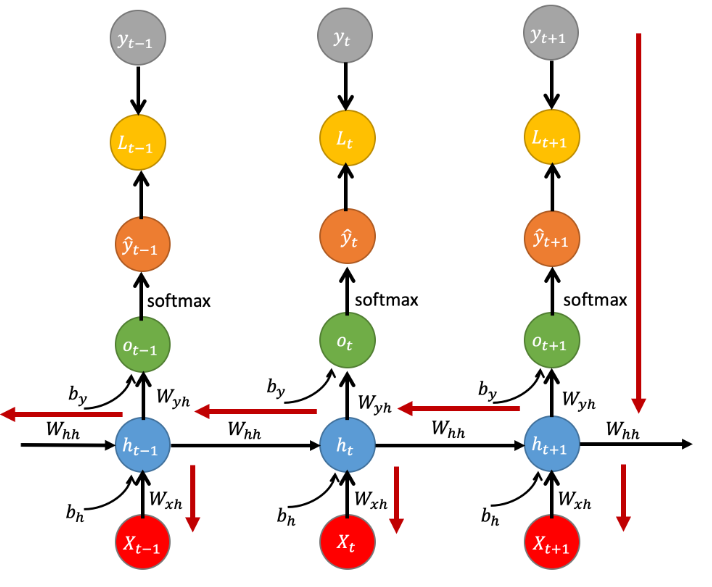
\includegraphics[width=0.8\textwidth]{rnn.png}
    \caption*{Unfolded Recurrent Neural Net} (Credit: \cite{murat_bptt})
    \label{fig: rnn}
\end{figure}

In this document, we shall derive gradient of the loss of RNN
w.r.t. the \textit{hidden weights} $W_{hh}$. In truth, we shall
derive the gradient aka differentiate the \textbf{loss at a particular
time instant wrt \textit{the concatenated weight matrix $[W_{xh}\;W_{hh}]^T$}}
This concatenation does not make any difference from a computational
perspective. \cite{d2l_bptt, murat_bptt}.

The emprical loss of the neural network is,

\begin{equation}
    \hat{L} = \frac{1}{T} \sum_{t=1}^{T} \ell(y_t, d_t) = \frac{1}{T} (l_1 + l_2 + ... + l_t ... + l_T)
\end{equation}

For an RNN, the system is defined by,
\begin{align}
    h_{t} &= f (X_{t}, h_{t-1}) = \phi_{h}(W_{xh} \cdot X_{t} + W_{hh}\cdot h_{t-1} +b_{h}) \\
    \hat{o}_{t} &= f_{o}(h_{t}) = \phi_{o}(W_{hy}\cdot h_{t} + b_{y})
\end{align}

Let $w_h = [W_{xh}\;W_{hh}]^T$.

Thus,

\begin{equation}
    \frac{\partial \hat{L}}{\partial w_h} = \frac{1}{T} (\frac{\partial l_1}{\partial w_h} + \frac{\partial l_2}{\partial w_h} + ... + \frac{\partial l_t}{\partial w_h} ... + \frac{\partial l_T}{\partial w_h})
\end{equation}

Now the loss at a particular time instant t follows the chain rule of derivatives.

\begin{equation}
    \frac{\partial l_t}{\partial w_h} = \frac{\partial l_t}{\partial o_t}\frac{\partial o_t}{\partial h_t}\frac{\partial h_t}{\partial w_h}
    \label{eq: l_t}
\end{equation}

But $h_t$ is a function of $h_{t-1}$ and $w_h$ as well (besides $X_t$).
Furthermore, $h_{t-1}$ is again a function of $w_h$.
Thus, by the multivariable chain rule,

If $h_t = f_1(h_{t-1}, w_h), h_{t-1}= g_1(h_{t-2}, w_h), w_h = h_1(w_h)$ \footnote{(Note: $h_1$ (the function, \textit{not} the hidden state) is merely the identity
function. We've formulated it so just to be consistent with the
formulation of "case 1" in \cite{multivariate_chain_rule}. Eqn \ref{eq: h_t wrt wh} would still 
be valid even if we hadn't defined it as a separate function.}

\begin{equation}
    \frac{\partial h_t}{\partial w_h} = \frac{\partial f_1}{\partial w_h} + \frac{\partial f_1}{\partial h_{t-1}}\frac{\partial h_{t-1}}{\partial w_h}
    \label{eq: h_t wrt wh}
\end{equation}

Similarly, if $h_{t-1} = f_2(h_{t-2}, w_h), h_{t-2}= g_2(h_{t-3}, w_h), w_h = h_2(w_h)$

\begin{equation}
    \frac{\partial h_{t-1}}{\partial w_h} = \frac{\partial f_2}{\partial w_h} + \frac{\partial f_2}{\partial h_{t-2}}\frac{\partial h_{t-2}}{\partial w_h}
\end{equation}

Similarly, if $h_{t-2} = f_3(h_{t-3}, w_h), h_{t-3}= g_3(h_{t-4}, w_h), w_h = h_3(w_h)$

\begin{equation}
    \frac{\partial h_{t-2}}{\partial w_h} = \frac{\partial f_3}{\partial w_h} + \frac{\partial f_3}{\partial h_{t-3}}\frac{\partial h_{t-3}}{\partial w_h}
    \label{eq: h_t-2 wrt wh}
\end{equation}

We can find similar expressions for time steps further back $h_{t-3}, h_{t-4}$ all the way to $h_1$.

Thus, eqn \ref{eq: h_t wrt wh} becomes, 

\begin{align}
    \frac{\partial h_t}{\partial w_h} &= \frac{\partial f_1}{\partial w_h} + \frac{\partial f_1}{\partial h_{t-1}}(\frac{\partial f_2}{\partial w_h} + \frac{\partial f_2}{\partial h_{t-2}}\frac{\partial h_{t-2}}{\partial w_h}) && (\text{we won't expand $\frac{\partial h_{t-2}}{\partial w_h}$}) \\
                                      &= \frac{\partial f_1}{\partial w_h} + \frac{\partial f_1}{\partial h_{t-1}}\frac{\partial f_2}{\partial w_h} + \frac{\partial f_1}{\partial h_{t-1}}\frac{\partial f_2}{\partial h_{t-2}}\frac{\partial h_{t-2}}{\partial w_h} \\
                                      &= \frac{\partial h_t}{\partial w_h} + \frac{\partial h_t}{\partial h_{t-1}}\frac{\partial h_{t-1}}{\partial w_h} + \frac{\partial h_t}{\partial h_{t-1}}\frac{\partial h_{t-1}}{\partial h_{t-2}}\frac{\partial h_{t-2}}{\partial w_h}
\end{align}

Now, we need to expand $\frac{\partial h_{t-2}}{\partial w_h}$ using eqn \ref{eq: h_t-2 wrt wh} to get the final
form but we can instead write it more compactly by realizing that this equation is ultimately 
a \textbf{summation of multiplications}. Let's break it down next.

\textbf{What are the terms of the summation?} Observe that every term's last (right-most) term is 
partial of $h_i$ and $i$ progresses from the beginning and ends at $t$ as we move from right to left
in the summation. Hence, $i$ is our index of summation. Now, every term is again a cascade of 
multiplications, decreasing in  number of multipliers as we move from right to left in the summation.
Every multiplier term is a partial of $h_j$ wrt $h_{j-1}$. (If our index of multiplication was $i$, as it was for the summation, each summation term would be different from
those found in eqn \ref{eq: h_t wrt wh}.)

Thus, the final form of \ref{eq: h_t wrt wh} can be written as,

\[
\boxed{\frac{\partial h_t}{\partial w_h} = \frac{\partial h_t}{\partial w_h} + \sum_{i=1}^{t-1}\prod_{j-1=i}^{t} (\frac{\partial h_j}{\partial h_{j-1}}) \frac{\partial h_i}{\partial w_h}
}
\]

Which is the same as equation 9.7.7 in \cite{d2l_bptt}.

\printbibliography

\end{document}